% ---------------------------------------------------------------------------
% \subsection{Computational Challenges}

Most advances in high-performance computing have focused on the scale,
performance and optimization of single long simulations. Due to the end of
Dennard scaling and methodological advances, many applications are now
formulated using multiple, shorter ensemble-based simulations. There are
however, limited software solutions that can support the scalable execution of
multiple tasks concurrently.

HTBAC has three primary design requirements\@: (1) enable the scalable
execution of concurrent multi-stage pipelines, flexibily partitioned across
different prototocols, (2) abstract the complexity of building protocols,
execution and resource management; and, (3) provide adaptive features (i.e.,
modifiying the task-graph during runtime, based on previous tasks), to enable
efficient protocols and effective resource sharing across protocols, without
explicit resource management requirements.

% In principle, many workflow management systems (WMS) can be used to express
% ensemble-based workflows to compute binding free energies. General-purpose WMS
% are however,  limited by a lack of specificity: workflow system with feature
% rich, but complex interface models impose substantial overhead when
% integrating application workflows in the runtime system, preventing users from
% quick and flexible applications prototyping.

% Furthermore, statistically meaningful results derived from simulations are of
% critical interest, as they can leverage additional sampling of simulations
% which could lead to an improvement in precision of free energy calculations.
% Such decisions typically, cannot be made {\it a priori} and require postmortem
% user intervention in order to analyze and spawn additional simulations.
% Specific features such as steering and adaptivity (e.g., spawning additional
% simulations) during runtime often require a redistribution of resources.
% Current WMS do not provide adequate support for dynamic resource utilization
% and require special extensions for adaptive formulations thus limiting the
% possibility of adaptive workflows.

HTBAC builds upon established middleware solutions~\cite{review_bb_2016},
validated runtime abstractions~\cite{turilli2017comprehensive} for scalable
execution of heterogeneous computational tasks, and customizes them for the
computation of binding free energies. HTBAC derives many of the advantages of
a lightweight, flexible domain specific workflow layer from its use of
RADICAL-Cybertools (RCT) which are functionally well-defined and delineated
middleware building blocks. RCT~\cite{review_bb_2016} are engineered to
support extensible and scalable workflows across diverse computing platforms.
The two primary RCT components that HTBAC depends upon are the Ensemble
Toolkit (EnTK) and RADICAL-Pilot (RP).  Figure~\ref{fig:integration} shows the
layered architecture of HTBAC, EnTK, and RP.

% HTBAC is implemented in Python, and uses RCT to provide ensemble-execution
% capabilities and a runtime system to execute tasks. 

EnTK simplifies the process of creating ensemble-based applications with
complex coordination and communication requirements. The EnTK API exposes the
PST model which consists of three components: \textbf{Pipeline},
\textbf{Stage}, and \textbf{Task}. HTBAC promotes binding affinity  {\bf
Protocols} as the user-facing construct, and also uses the programming model
defined by the Pipeline, Stage and Tasks model to express a variety of
protocols: each stage is a computational \textbf{task}, and the
ordered aggregation of these stages alongside their dependencies as a
\textbf{pipeline}. A workflow is comprised of $N_P$ instances of the P$^{th}$
protocol.

The \textbf{Protocol} class can be instantiated as one of two protocols: ESMACS or TIES. For
TIES, each protocol typically corresponds to a single physical system, and
multiple instances can be supported. The TIES protocol object enables the user
to select a physical system, number of replicas, core allocation per replica,
and $\lambda$ windows to sample. Figure~\ref{fig:pst}
provides the visual implementation of the TIES protocols into the PST model.

% Consistent with EnTK's programming model, HTBAC also uses the PST model to
% express {\bf Protocols}.

% Each protocol contains multiple stages with simulations and analysis tasks
% interspersed, in the most general case. 


% programming model (that are consistent with the EnTK) to enable the user 

% In section \ref{sec:science-drivers}, we described two examples of ensemble-
% based protocols for computing binding affinities.

% (so far, a
% workflow entails a maximum value of $P = 2$ and $N_P$=16, but in future work P
% will be greater $>$ 2).

Once the workflow is described, it is submitted to EnTK's
\textbf{Application Manager} which sets up multiple processes, threads and a
RabbitMQ message queue for communication.
EnTK identifies tasks which have satisfied dependencies and can be executed
concurrently. EnTK's \textbf{Execution Manager} uses the underlying runtime
system, RADICAL-Pilot to execute the tasks on specific target resources.

\begin{figure}
  \centering
   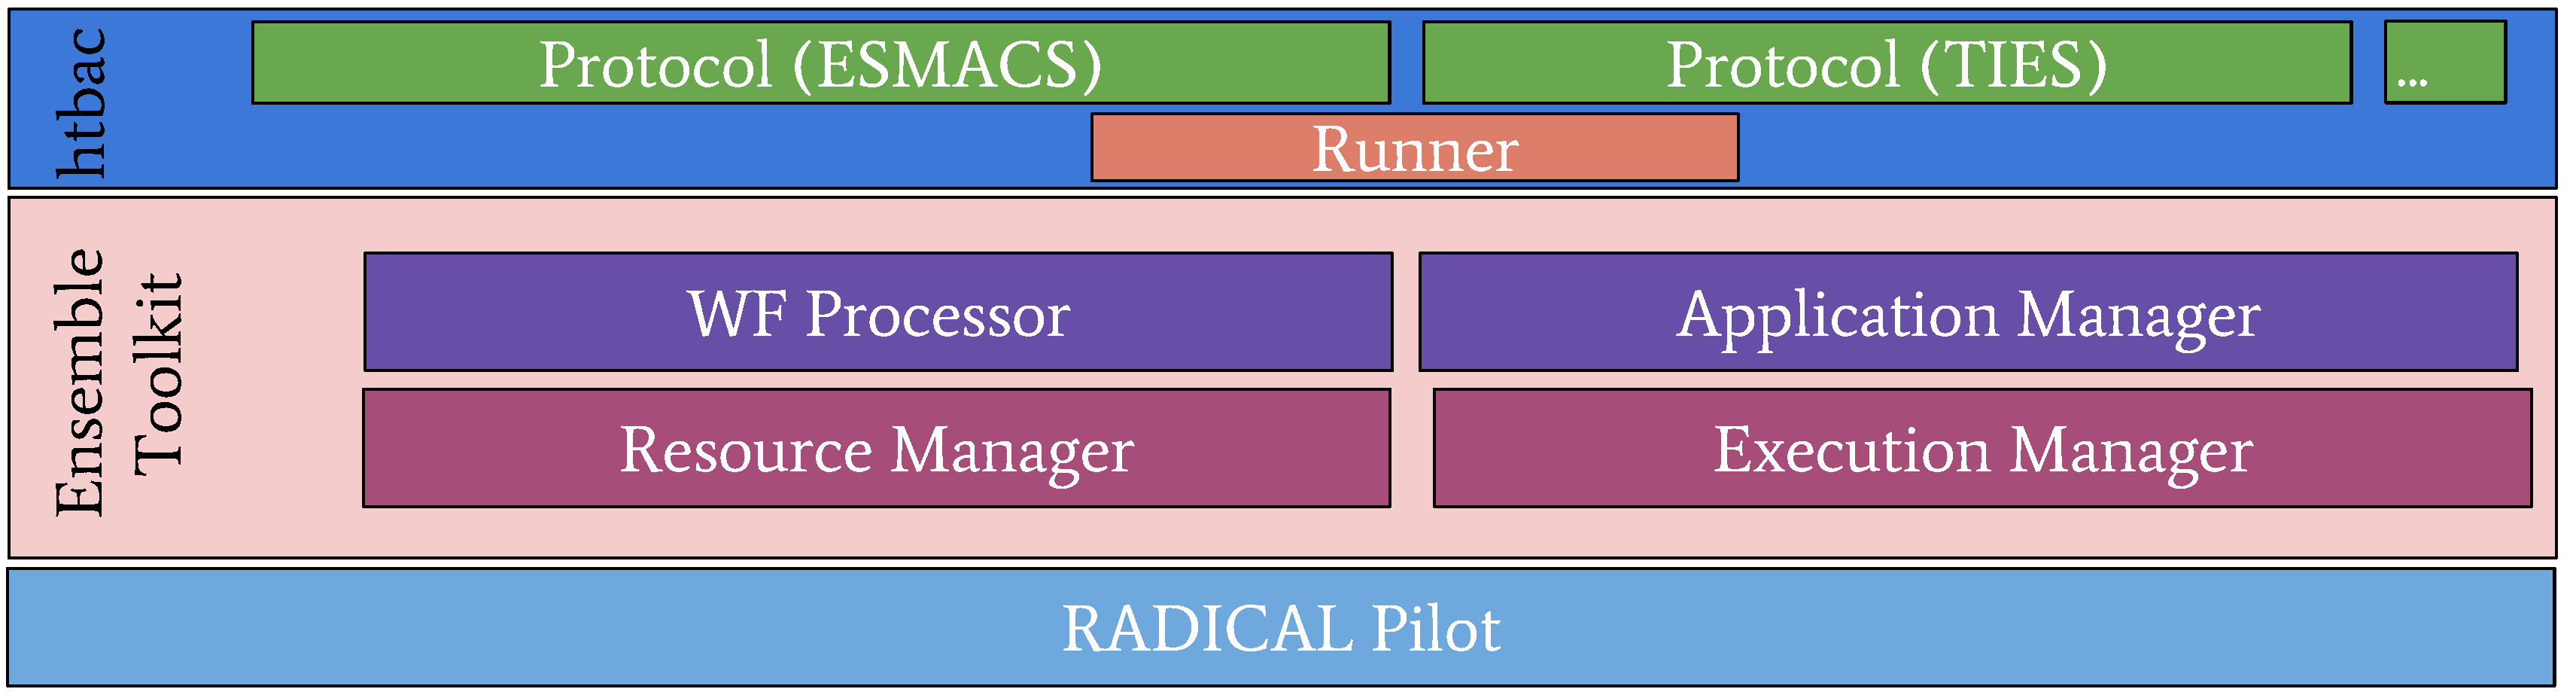
\includegraphics[width=\columnwidth]{figures/isc_htbac_integration_with_entk_RP.pdf}
  \caption{Layered architecture of HTBAC, EnTK, and RP. The HTBAC API exposes the Protocol
  component. Current protocols supporting the use cases include ESMACS/TIES.  
  EnTK serves as the workflow execution system, and by managing the workflow and workload. 
  RADICAL-Pilot serves as the runtime system.}
\label{fig:integration}
\end{figure}

% protocol, a user can scale protocol instances to study as many physical systems as
% desired.

% The specification of protocols and their parameters are passed by the user to
% the \textbf{Runner Handle} which translates the request to EnTK.

In Section \ref{sec:related-work} we highlighted how an ensemble
simulation approach can both aid sampling and improve uncertainty
quantification for free energy calculations. Despite these crucial advantages,
it remains non-trivial for field researchers to write biosimulation
applications that involve individual protocols supporting multiple replicas,
and by extension multiple protocols. With HTBAC, this burden is minimized by
specifying the number of concurrent instances of the \textbf{Protocol} object.
Moreover, the ability to generate multiple protocol instances enables the user
to investigate a range of physical systems (i.e., drug candidates)
concurrently.

HTBAC allows the simple expression and concurrent execution of multiple
distinct protocols, thereby enabling concurrent screening of drug candidates.
HTBAC not only simplifies the expression of complex binding affinity
protocols, but also provides hitherto unavailable capabilities, viz., the
adaptive execution of these protocols, without any additional programming
burden. 


% In turn, our adaptive execution implementation at the WMS focuses on
% supporting generality of adaptive workflows at the inter and intra-protocol
% level.

\begin{figure}
  \centering
   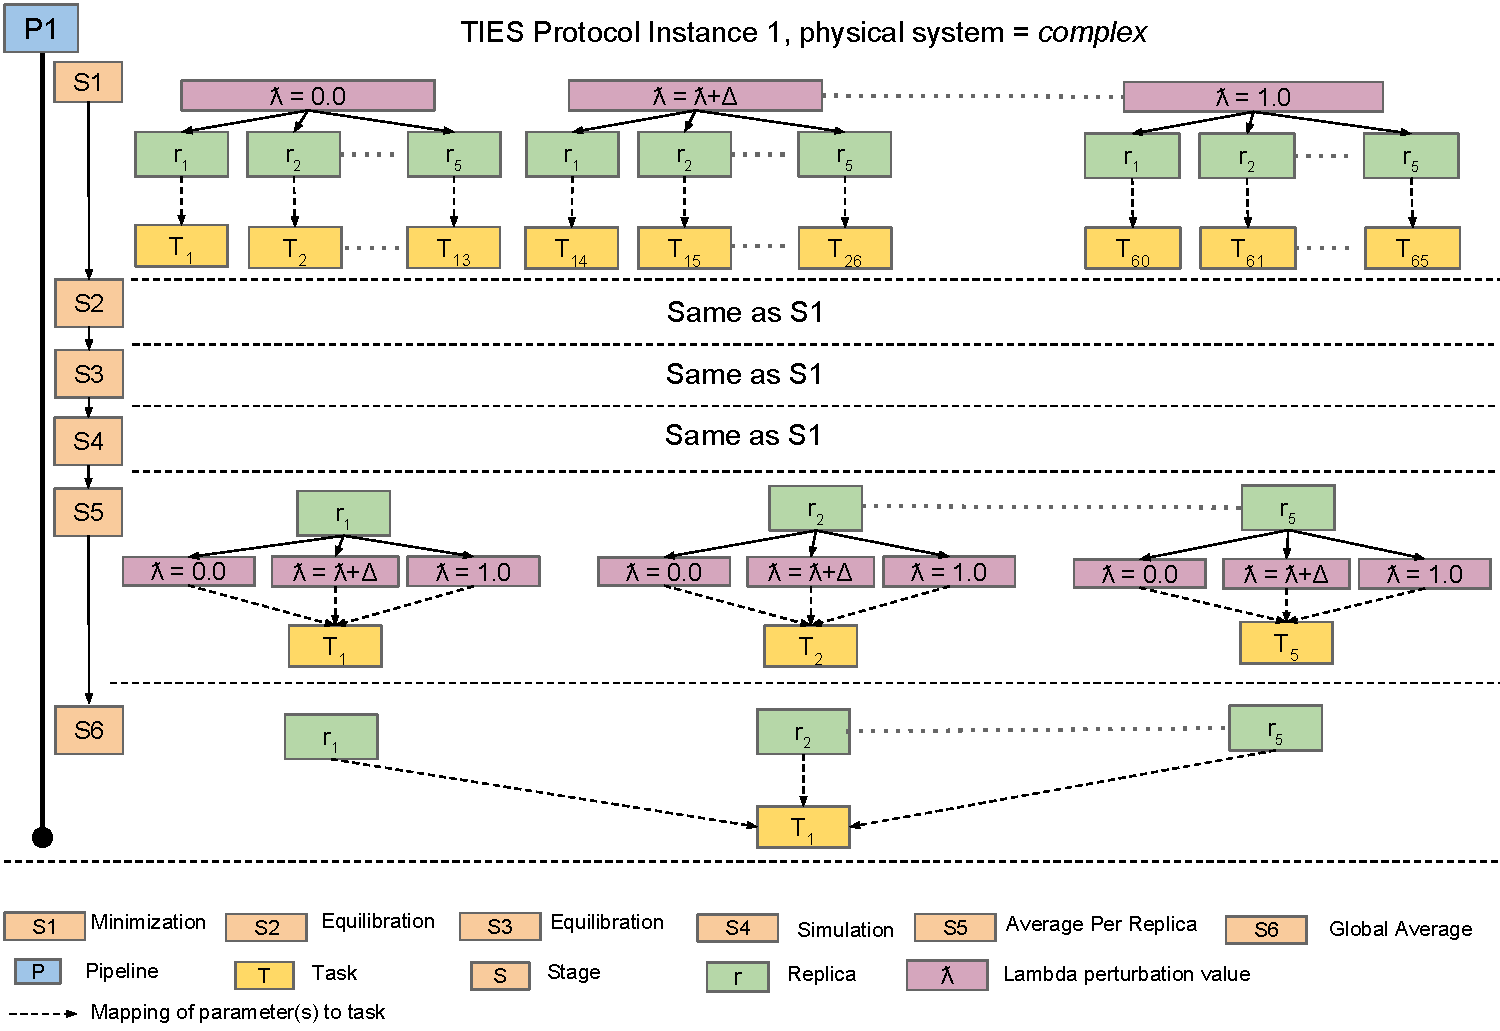
\includegraphics[width=\columnwidth]{figures/_TIES_EnTK_implementation.pdf}
  \caption{TIES protocol expressed using the EnTK PST model. Each protocol 
  instance maps to a single Pipeline, comprised of Stage(s) which maintain 
  temporal order. Each Stage executes $n$ tasks, where $n$ represents the 
  number of unique lambda-replica combinations.}
\label{fig:pst}
\end{figure}

In section \ref{sec:science-drivers}, we described a particular type of
adaptivity within TIES that would enable the simulation to reach
convergence earlier. Adaptive execution requires changes to the taskgraph 
during runtime, capabilties that are supported by the RCT runtime layers~\cite{power-of-many17}.

The TIES adaptive workflow decides, post-mortem, about the placement
of new lambda windows for the next set of simulations. In turn this requires task-
count adaptivity which we define as runtime changes to the number of tasks in
the taskgraph. HTBAC monitors the output results from the completed tasks
during runtime, and redefines the existing workflow by adding more $\lambda$
windows. Using EnTK, HTBAC creates the necessary set of
new tasks. The \textbf{Application
Manager} in EnTK signals RP to bypass termination of the pilot and instead
keep the session alive, as long as additional tasks are submitted. As the
number of tasks grow during runtime, the ratio of core-to-task will fluctuate.
HTBAC exposes the core allocation per task, and allows the user control to
pre-specify resource requirements of additional tasks.

% ---------------------------------------------------------------------------


%\jhanote{Is this specific to the TIES protocol or to the protocol class. Needs
%clarification.}
%The same approach has been expanded to facilitate the creation of
%sub-ensembles where the simulation configuration is altered programatically.
%An example of this is the implementation ofthe TIES protocol,
%where the user controls the $\lambda$ parameter values used in simulatios to
%control which hybrid system states are sampled.

%A parameter, $\lambda \in [0, 1]$ is set for values between extremes and a
%simulation has to be run for every $\lambda$ value. The values form a function
%of energy and are integrated to obtain the desired results, the
%\emph{relative} binding free energy.

%\subsubsection{System}

%Systems This allows for multiple systems to be tested in the same
%\emph{single} run. A common scenario is the calculations of the binding
%affinity of a set of ligands with the same protein. System itself is just a
%collection of file paths pointing to descriptions of the system, like the
%system structure, topology etc. This class also provides the core/node
%requirments per single run, and reads some of the system descriptions from
%files to fill in the configuration settings.

%The Pipeline-Stage-Task (PST) framework developed by the Radical team
%(cite), and the Ensemble Toolkit (EnTK) built on top of it, offers a
%flexible way to express the molecular dynamics simulation workflows present
%in academia (cite) in terms of the radical pilot execution environment. Here
%we present a proposed mapping between the two (the PST and the MD layers)
%that is both simulation engine and protocol agnostic and allows for the
%compact expression of ensembles frequently used in binding affinity
%calculations.

%\subsection{Overview}

%The framework, called High Throughput Binding Affinity Calculator (HT-BAC),
%a python library, is made up of the following components: Workflow, Step,
%Ensembles and Simulation. These four object are all that is neccessary to
%describe the complex binding affinity caluculations in a generic way.

%\subsection{Workflow}

%The highest level abstraction is the Workflow. It is a container for the
%sequential units that are the simulation steps themselfs, and also contains
%meta-information about the job, like the resource description that the job
%will be running on, the total number of cores (nodes) required to fullfil
%the needs of the simulations and profiling mechanims to measure execution
%time.

% ---------------------------------------------------------------------------
%\jhanote{I don't these "description" should be subsections. Consider
%"\paragraph{}"}

%\subsection{Step}

%\jhanote{what is a step? It is unclear to the reader. Is "step"  construct
%within HTBAC or is this just a description of the pipeline?}

%The workflow containts an ordered list of \emph{steps}. Steps give
%\jhanote{order?} orderd to the basic building blocks of binding affinity
%calculations. Usually they are (i) minimization (some form of local
%optimization of atom coordinates), (ii) heating, (iii) equilibration and (iv)
%production run.

%Additionally there is one or more steps of analysis at the end. The key
%point, is that these steps \emph{have} to be run consecutively, as they are
%dependent on the previous one. This is ensured by the \texttt{Stage} objects
%of EnTK\@. Each step has list of \texttt{Ensemble}s and a \texttt{Simulation}
%object.

% ---------------------------------------------------------------------------

%$\subsection{Adaptability}

%Once we tackle the barrier between the local workflow creation and the remote
%execution, new features become availble, and readily usable by scientists.
%Intraprotocol adaptability is one such new feature.

% ---------------------------------------------------------------------------

% \subsubsection{Intraprotocol adaptability}

%while conceptually simple, tradiational execution patters used in academia
%makes this very hard. In HTBAC variables like replica size, specific lambda
%windows or simulatable system are settable on demand, the execution of which
%is automatically handeled by the library. To illustrate: a common scenario is
%the non adequate convergence of the statistical results after running a given
%number of replicas. In HTBAC the replica number can be changed, rerun and the
%results reevaluated. Additionally, logic can be written, to dynamically add
%more replicas until a given convergence tolerance has been reached.
